\documentclass[a4paper,12pt,french]{book}
\usepackage[margin=2cm]{geometry}
\usepackage[thinfonts]{uglix2}

\setminted{fontsize=\small}\nouveaustyle
\begin{document}
\titre{BDD partie 4 - Exercices}{NSI2}{2021}


\begin{exercice}[ : Prix Nobel]
\begin{center}
	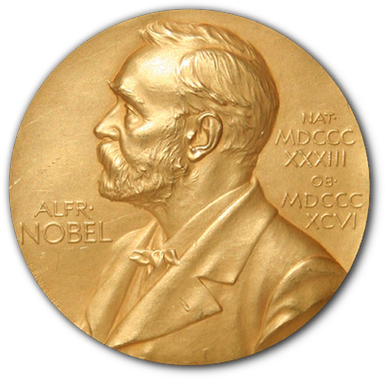
\includegraphics[width=5cm]{img/nobel}
\end{center}
\textbf{Premier contact}\\

Avec un éditeur de texte ouvir le fichier \texttt{create\_nobel.sql}.\\
En explorant la structure de la base de données, répondez aux questions suivantes :	\\
\begin{enumerate}[\bfseries 1.]
	\item 	Combien de tables possède la base de données ?
	\item 	Combien d’attributs possède la table Nobel ?
	\item 	Quel est le type de l’attribut annee ?\\
\end{enumerate}
\textbf{La table Nobel}\\

Importer ce fichier dans DB Browser pour créer la BDD \texttt{nobel.db}.\\
En explorant les données de la table Nobel, répondez aux questions suivantes :\\

\begin{enumerate}[\bfseries 1.]
	\setcounter{enumi}{3}
	\item 	Combien d’enregistrements possède la table Nobel ?
	\item 	Dans quelle discipline Paul Krugman est-il devenu Prix Nobel ?
	\item 	En quelle année Albert Fert a-t-il eu le prix Nobel ?	\\
\end{enumerate}
\newpage
\textbf{Requêtes d'interrogation}\\

En utilisant l’onglet : \og Exécuter le SQL \fg, indiquez le code SQL permettant de répondre aux questions suivantes :\\

\begin{enumerate}[\bfseries 1.]
		\setcounter{enumi}{6}
\item  Comment afficher le nom de tous les lauréats en évitant les doublons ? (809 enregistrements)
\item Comment afficher le nom de toutes les disciplines en évitant les doublons ? (6 enregistrements)
\item  Quelle est la discipline de Wilhelm Conrad Röntgen ? (1 enregistrement)
\item  Dans quelle discipline Paul Krugman est-il devenu Prix Nobel ? (1 enregistrement)
\item  En quelle année Albert Fert a-t-il eu le prix Nobel ? (1 enregistrement)
\item  Quelle est l’année de distinction de Pierre Curie ? (1 enregistrement)
\item  Quelle est l’année de distinction et la matière de Bertha von Suttner ? (1 enregistrement)
\item  Quels sont les lauréats distingués au XXI e siècle ? (97 enregistrements)
\item  Quels sont les lauréats du prix Nobel de la Paix durant la deuxième guerre mondiale ? (2 enregistrements)
\item  Quels sont les lauréats distingués en Médecine en 1901 et en 2001 ? (4 enregistrements)
\item  Quels sont les lauréats des prix nobel de Physique et de Médecine en 2008 ? (3 enregistrements)	\\
\end{enumerate}

\textbf{Requêtes d'agrégation}\\

\begin{enumerate}[\bfseries 1.]

\item  Combien d’enregistrements au total comporte la table ? (816 enregistrements)
\item  Combien de personnes ont reçu le prix Nobel de la paix ? (119 enregistrements)
\item  Combien de personnes ont reçu le prix Nobel de littérature ? (105 enregistrements)
\item  Combien de personnes ont reçu le prix Nobel de mathématiques ? (0 enregistrements)
\item  Combien de personnes ont reçu un prix Nobel en 1901 ? (6 enregistrements)
\item  Combien de personnes ont reçu un prix Nobel de chimie en 1939 ? (2 enregistrements)
\item  En quelle année a été décerné le premier prix Nobel d’économie ? (Réponse : 1969)
\item  Combien de prix Nobel a reçu Marie Curie ? (Réponse : 2)
\item  Quels sont les prix lauréats, leur discipline et l’année de distinction de tous les prix Nobel contenant cohen dans leur nom (on ne fera pas de distinction de casse) ? (2 enregistrements)
\item  Combien y a-t-il eu de lauréats en Physique et en Chimie ? (335 enregistrements)
\item  Combien y a-t-il eu de lauréats de Médecine et de littérature en 2000 ? (4 enregistrements)
\item  Nombre de lauréats différents parmi les prix Nobel de la paix ? (116 enregistrements)\\
\end{enumerate}

\textbf{Requêtes de mise à jour}\\

En utilisant l’onglet Exécuter le SQL, indiquez le code SQL permettant de répondre aux questions suivantes :\\

\begin{enumerate}[\bfseries 1.]
\item En 2019, Esther Duflo a reçu le prix Nobel d’économie. Écrivez la requête permettant d’insérer cet enregistrement.
\item  Quelle requête permet de modifier l’enregistrement précédent pour accoler le nom d’époux (Banerjee) après celui de Duflo ?
\item   De nombreuses pétitions circulent pour retirer le prix Nobel à Aung San Suu Kyi. Quelle requête permettrait cela ?
\end{enumerate}
\end{exercice}



\begin{exercice}[ : Collectivites.db]

\textbf{Exploration de la base}\\

En explorant la structure de la base de données, répondez aux questions suivantes :

\begin{enumerate}[\bfseries 1.]
	\item 	Combien de tables possède la base de données ?
	\item 	Pour la table \textbf{Departement}
	\begin{enumerate}[\bfseries a.]
		\item 	Identifiez le type de chaque attribut.
		\item 	Quelle est la clé primaire ?
	\end{enumerate}
	\item Pour la table \textbf{Ville}
		\begin{enumerate}[\bfseries a.]
		\item 	Identifiez le type de chaque attribut.
		\item 	Quelle est la clé primaire ?
		\item 	Quelle est la clé étrangère et quel attribut référence-t-elle ?
	\end{enumerate}
	\item 	 Réalisez un schéma relationnel de cette base de données, sous la forme graphique, en précisant pour chaque attribut son type et s’il doit impérativement être rempli.
\end{enumerate}


\textbf{Collecte des informations}\\

La base \textbf{Collectivites} est vide. Il faut la remplir. Pour cela, en vous aidant de Wikipedia, complétez les tableaux suivants.
C'est à vous de remplir comme bon vous semble les colonnes idCommune et idDepartement.
\begin{center}
\begin{tabular}{|c|c|c|c|c|}
	\hline
	\rowcolor{UGLiOrange}\color{white} idCommune &\color{white}	\textbf{Commune} & \color{white}\textbf{Code postal} & \color{white}\textbf{Département} &\color{white} \textbf{Nombre d'habitants} \\
	\hline\color{black}
	&Rouen &  &  &  \\
	\hline
	&Dieppe &  &  &  \\
	\hline
	&Envermeu &  &  &  \\
	\hline
	&Le Neubourg &  &  &  \\
	\hline
	&Igoville &  &  &  \\
	\hline
\end{tabular}\\[1em]

\begin{tabular}{|c|c|c|}
	\hline
\rowcolor{UGLiOrange}\color{white} idDepartement &\color{white}	\textbf{Département} & \color{white}\textbf{Code d'immatriculation} \\
	\hline
	&Seine-Maritime  & \\
	\hline
	&Eure&  \\
\hline
	&Calvados&  \\
\hline

\end{tabular}
\end{center}

\textbf{Exploitation des informations}\\

En utilisant l’onglet \og Exécuter le SQL\fg{}, indiquez le code SQL permettant de répondre aux consignes suivantes :\\
\begin{enumerate}[\bfseries 1.]
	\setcounter{enumi}{4}
	\item 	Insérez le département de Seine-Maritime.
	\item 	Insérez la commune de Rouen.
	\item 	Faîtes de même, en une seule requête, avec les communes de Dieppe et d’Envermeu.
	\item 	Insérez la commune d’Igoville.
	\item 	Insérez la commune du Neubourg.	\\
\end{enumerate}
En recherchant éventuellement les informations manquantes, indiquez le code SQL permettant de répondre aux consignes suivantes :\\
\begin{enumerate}[\bfseries 1.]
		\setcounter{enumi}{9}
	\item 	Trouville, Mézidon-Canon et Crèvecoeur-en-Auge sont des villes du Calvados.
	\item 	Le vrai nom de Trouville est en fait Trouville-Sur-Mer.
	\item 	Médizon-Canon et Crèvecoeur-en-Auge n’existent plus. Elles ont fusionné pour donner une nouvelle commune : Mézidon-Vallée-d’Auge.\\
\end{enumerate}
\textbf{Vérification des données}\\

En trouvant les requêtes SQL adéquates, répondez aux questions suivantes.

\begin{enumerate}[\bfseries 1.]
	\setcounter{enumi}{12}
\item  Combien il y a-t-il de départements différents enregistrés dans la base ? (réponse : 3)
\item Combien il y a-t-il de communes différentes enregistrées dans la base ? (réponse : 7)
\item Combien il y a-t-il de communes dans l’Eure enregistrées dans la base ? (réponse : 2)
\item  Combien il y a-t-il de communes en Seine-Maritime enregistrées dans la base ? (réponse : 3)
\item Combien il y a-t-il de communes dans le Calvados enregistrées dans la base ? (réponse : 1)
\end{enumerate}
\end{exercice}





\begin{exercice}[ : JO]
Nous allons travailler sur une base de données liée aux Jeux Olympiques de Londres qui ont eu lieu en 2012.\\
\begin{center}
	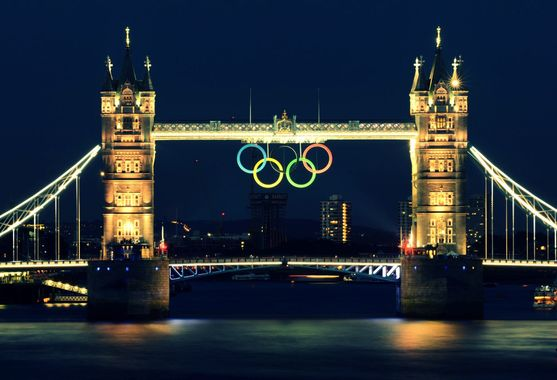
\includegraphics[width=8cm]{img/jo_london}
\end{center}

\textbf{\large Partie 1 : \'Etude du schéma relationnel}\\

Avec un éditeur de texte tout simple, ouvrir le fichier \texttt{create\_JO.sql}, regarder les lignes qui définissent les différentes tables de la BDD et donner sous forme écrite son schéma relationnel en soulignant clés primaires (en trait plein) et clés étrangère (en pointillés).\\

\textbf{\large Partie 2 : Requêtes SQL}\\

Avant toute chose, ouvrir DB Browser, importer le fichier \texttt{create\_JO.sql} pour créer la BDD \texttt{JO.db}.\\
Ensuite exécuter les bonnes requêtes SQL pour obtenir les données suivantes.\\

\textbf{Requêtes sans jointures}
\begin{enumerate}[\bfseries 1.]
	\item 	Afficher le nom et prénom des sportifs. Combien y en a-t-il ?
	\item 	Afficher les codes des pays dont viennent les sportifs par ordre alphabétique en éliminant les doublons.
	\item 	Afficher la liste des sportifs français (utiliser cio = 'France').
	\item 	Afficher la liste des 301 disciplines triées par l'identifiant du sport auxquelles elles se rapportent.
	\item 	Afficher les noms des 86 pays situés après la France et avant la Russie (Russia) par ordre alphabétique.\\
			Utiliser les opérateurs inférieur et supérieur. Remarquer que l'opérateur \mintinline{SQL}{BETWEEN} ne produit pas le résultat attendu (88 pays).
	\item 	Afficher les 98 identifiants de discipline dont au moins une épreuve a eu lieu entre le 27 et le 31 juillet 2012 inclus.
	\item 	Afficher les noms des 61 sportifs qui sont soit français (FRA) soit britanniques (GBR).
	\item 	Afficher les intitulés des 131 disciplines contenant la chaîne de caractères «WOMEN».

	\item  Donner les 3 pays (CIO, nom) dont on ne connaît pas le code ISO2 ou ISO3 (utiliser le critère \mintinline{sql}{IS NULL}).
	\item 	Donner les noms et prénoms des 2 sportifs dont le sexe est mentionné dans la BDD.
	\item  	À l'aide de la fonction \mintinline{sql}{COUNT}, donner le nombre de sports (pas la liste).
	\item  Donner le nombre de discipline(s) du sport d'identifiant 1 (pas la liste).


	\item Combien de noms de familles différents sont portés par les sportifs ?
	\item Donner le nombre de pays n'ont pas d'ISO2.
	\item Donner le nombre de médailles d'or attribués lors de ces JO.
	\item Afficher en une table le premier et le dernier évènement sportif	de ces JO.
\end{enumerate}
\textbf{Requêtes avec jointures}
\begin{enumerate}[\bfseries 1.]
	\setcounter{enumi}{16}
	\item Afficher la listes des noms et prénoms des sportifs européens.
\item Afficher la liste des disciplines dépendant de l'athlétisme.
\item Afficher toutes jours pendant lesquels un évènement lié à l'athlétisme eu lieu.
\item Afficher les noms, prénoms et médailles gagnées par des sportifs dont le sexe figure dans la BDD.
\item Afficher la liste des Français médaillés d'or.
\item Afficher les noms, prénoms, sports et disciplines des sportifs ayant obtenu une médaille d'or.
\end{enumerate}

\end{exercice}
\end{document}